%This template is based on one provided by the American Physical Society for submission to its journals.

\documentclass[aps,twocolumn,showpacs,preprintnumbers]{revtex4}

%The following packages add LaTeX commands that make formatting and writing math easier

\usepackage{graphicx}  % Include figure files
\usepackage{subfigure}
\usepackage{multirow}

\linespread{1.1}
\usepackage{fancyhdr}
\usepackage{longtable}
\usepackage{parskip}
\usepackage[T1]{fontenc}
\usepackage{dcolumn}   % Align table columns on decimal point

\usepackage{bm}        % bold math
\usepackage{amsfonts}  % Common math fonts
\usepackage{amsmath}   % Common math functions
\usepackage{amssymb}   % Common math symbols

%The following custom commands simplify commonly used LaTeX commands

\newcommand{\pic}[2]{\begin{center} \includegraphics[scale=#1]{#2}\end{center}}
\newcommand{\re}[1]{\mathrm{Re}\left(#1\right)}
\newcommand{\im}[1]{\mathrm{Im}\left(#1\right)}
\newcommand{\bdot}[1]{\dot{ \bb {#1}}}
\newcommand{\bddot}[1]{\ddot{ \bb {#1}}}
\newcommand{\bidot}[1]{\dot{ \bi{ #1}}}
\newcommand{\biddot}[1]{\ddot{ \bi {#1}}}
\newcommand{\ep}{\varepsilon}
\newcommand{\for}{\quad \quad \mathrm{for} \quad\quad}
\newcommand{\then}{\quad \quad \implies \quad\quad}
\newcommand{\an}{\quad \quad \mathrm{and} \quad\quad}
\newcommand{\ifff}{\quad \quad \mathrm{if} \quad\quad}
\newcommand{\where}{\quad \quad \mathrm{where} \quad\quad}
\newcommand{\dg}{^\dagger}
\newcommand{\semi}{\quad \quad \mathrm{;} \quad\quad}
\newcommand{\paren}[1]{\left( #1 \right)}
\newcommand{\brac}[1]{\left[ #1 \right]}
\newcommand{\bra}[1]{\left\langle #1 \right|}
\newcommand{\exv}[1]{\left\langle #1 \right\rangle}
\newcommand{\pwisein}{\left\{ \begin{array}{ll}}
\newcommand{\pwiseout}{\end{array}\right.}
\newcommand{\ket}[1]{\left| #1 \right\rangle}
\newcommand{\bracket}[2]{\left\langle #1 | #2 \right\rangle}
\newcommand{\trace}[1]{\mathrm{Tr} \left( #1 \right)}
\renewcommand{\det}[1]{\mathrm{det}\left( #1 \right)}
\newcommand{\del}[1]{\frac{\partial}{\partial #1}}
\newcommand{\fulld}[1]{\frac{d}{d #1}}
\newcommand{\fulldd}[2]{\frac{d #1}{d #2}}
\newcommand{\dell}[2]{\frac{\partial #1}{\partial #2}}
\newcommand{\delltwo}[2]{\frac{\partial^2 #1}{\partial #2 ^2}}
\newcommand{\bb}{\mathbf}
\newcommand{\bi}{\boldsymbol}
\newcommand{\eq}[1]{\begin{equation} #1 \end{equation}}
\newcommand{\radhalf}{ \frac{ \sqrt{2}}{2}}
\newcommand{\sigx}{\left( \begin{array}{cc} 0 & 1\\ 1 & 0 \end{array}\right)}
\newcommand{\sigy}{\left( \begin{array}{cc} 0 & -i\\ i & 0 \end{array}\right)}
\newcommand{\sigz}{\left( \begin{array}{cc} 1 & 0\\ 0 & -1 \end{array}\right)}
\renewcommand{\matrix}[1]{\left( \begin{array} #1 \end{array}\right)}
\newcommand{\thermo}[3]{\left( \frac{\partial #1}{\partial #2} \right)_{#3}}
\newcommand{\coolfrac}[2]{\left( \frac{ #1}{ #2} \right)}

\setlength{\parindent}{10pt}

\begin{document}

\title{Simulating the Mikheyev–Smirnov–Wolfenstein (MSW) effect \\ Neutrino oscillations in matter on a quantum computer}

\author{Baalateja Kataru}

\affiliation {\it School of Interwoven Arts and Sciences, \\Krea University, Sri City 517646, India}

\date{\today}

\begin{abstract}

%First sentence (or two) says something about the importance of the parameter being measured.
The viscosity of a particular fluid is an interesting parameter that plays an important role in fluid dynamics of that fluid. We chose the common household cooking item canola oil.
%The next sentence (or two) summarizes the measurement approach used.
Using a ball drop, we set out to measure viscosity at various temperatures and create a model for $\eta (T)$ between 0$^{\circ}$C and 100$^{\circ}$C, as well as an accurate measurement for viscosity at room temperature, $\eta (T=20^{\circ}$C).
%The final sentence (or two) state the result (measurement with its 68% confidence interval) and insight(s) concerning the measurement approach, if any.
It was found that the viscosity between 0$^{\circ}$C and 40$^{\circ}$C can be approximated using the function $\eta (T) = \alpha e^{-\beta T}$, where $\alpha = 440.65 \pm 30.40 \hspace{0.1cm} mPa\cdot s$ and $\beta = 0.03761 \hspace{0.1cm} \frac{1}{^{\circ}C}$ and that an estimation for viscosity at room temperature is equivalent to $207.6901\pm14.3306 \hspace{0.1cm} mPa\cdot s$.
The precision of this measurement was limited by uncertainty in lab equipment used to measure various quantities as well as the image analysis software we used and the limited frame-rate of our camera.

\end{abstract}

%For fun, see PACS list at  https://www.aip.org/publishing/pacs/pacs-2010-regular-edition
\pacs{47.15.-x}

\maketitle 

\section{Introduction}

%P1: Intro: scientific motivation

Quantum computers have long been touted as being new solutions to new problems. Apart from solving the longstanding challenges of cryptography, an important application of the power of quantum computers is to simulate physical systems. More specifically, quantum mechanical systems. This is due to the inherent quantum nature of the computers. In this era of Noisy Intermediate Scale Computing (NISQ), quantum computers have been used to simulate many physical systems. From variational eigensolvers to find ground eigenstates of the Hamiltonian in quantum chemistry, to improving the efficiency of the ammonia-producing Haber-Bosch process, NISQs are being used to tackle a variety of simulation problems previously considered intractable for a classical computer.

There is a much simpler quantum system that, rather surprisingly, has escaped being subjected to quantum simulation so far. The system in consideration is that of neutrino oscillations in matter. While there's no debate that this system has been thoroughly studied by methods of classical computing, neutrino oscillations may provide new insights into the behavior of neutrinos and other particles of the standard model when simulated on a quantum computer.

Neutrinos are tiny, subatomic particles that are produced in reactions such as nuclear decay and fusion processes at the heart of the sun. There are three types of neutrinos - the electron neutrino $\nu_e$, the muon neutrino $\nu_\mu$, and the tau neutrino $\nu_\tau$, one for each lepton in the standard model. Originally conceived by Enrico Fermi to account for the observation that momentum was not being conserved in the beta decay process, the solar neutrino problem of the late 20th century breathed new life into the study of these ghost-like particles, when it was discovered that neutrino flavor states are not eigenstates of the Hamiltonian, allowing neutrinos to oscillate amongst themselves as time passes.

\section{The theory of neutrino oscillations in vacuum}

\section{Quantum circuit for vacuum oscillations}

\section{The theory of neutrino oscillations in matter}

\section{Eigenvalue-Eigenvector and Adjugate identities}

The Trotter-Suzuki approximation

%P2: More intro: approach, definitions, history, context, rationale

We chose to measure the viscosity of canola oil as a function of temperature for a few reasons. For one thing, it was a convenient household item, and so we had easy access to large quantities of it. We wanted to develop it as a function of temperature because temperature varies significantly on a day to day basis, and so this is a commonly fluctuating variable that could change the properties of oil on a daily basis. We wanted to measure viscosity as a function of temperature between 0$^{\circ}$C and 100$^{\circ}$C as to have a more complete picture of the change in viscosity over temperature, but our data taken in the lab room was unusable as the camera we used was too low resolution and the frame-rate was too low. 

%P3: What you did, what you found 

Here I (we) report a simple approach to measuring the dynamic viscosity of canola oil as a function of temperature using a simple ball drop experiment.
% Another sentence or two describing important aspects of the approach.
This approach yielded a function of $\eta (T)$, and an estimate at room temperature for the viscosity of canola oil.
The precision of this measurement was limited by uncertainty in lab equipment used to measure various quantities, as well as the image analysis software we used and the limited frame-rate of our camera. 

\section{Theory}
Our calculation for viscosity will use the forces acting on a ball during a "ball drop" experiment, where a ball is dropped and the time taken to fall is measured. Viscosity is involved in one of the forces(Stokes' Drag)\cite{Chem_Book_Stokes_Drag} and so we can solve the corresponding equations for Viscosity.

We start out with an expression stating the various forces involved.

\begin{equation}\label{eq1}
F_{total} = \sum_{i=1}^{} F_{i} = F_{gravity} - F_{buoyant} - F_{stokes' drag}
\end{equation}

Now, making the substitutions\cite{RHK} that $F_{total}=ma$, $F_{gravity}=mg$, $F_{buoyant} = m_{disp}g$\cite{Footnote}, and $F_{stokes drag}=6\pi \eta Rv$, we can create the equation:

\begin{equation}\label{eq2}
ma = mg - m_{disp}g - 6\pi \eta Rv
\end{equation} 

Next we make the substitutions that $\Delta x=\frac{1}{2}at^2$ (and thus $a=\frac{2\Delta x}{t^2}$) and $v=\frac{\Delta x}{t}$.

\begin{equation}\label{eq3}
m\frac{2\Delta x}{t^2} = mg - m_{disp} - 6\pi \eta R\frac{\Delta x}{t}
\end{equation}

Now, we do some simple algebra to solve for $\eta$, as a function of our parameters $\Delta x$, $t$, $R$, $m$, and $m_{disp}$.

\begin{equation}\label{eq4}
\eta = \frac{mgt}{6\pi R \Delta x} - \frac{m_{disp}gt}{6\pi R \Delta x} - \frac{m}{3\pi Rt}
\end{equation}


\section{Approach}

%P4: Approach 1 - Setup (The nonsense below aims to give you a sense for style. It is purely imaginary.) 

Our approach was to place the canola oil into a standard household drinking glass, and to drop the ball from the top of the glass, and to measure the time taken for the ball to fall to the bottom. We varied the temperature of the oil by placing the drinking glass in a hot water bath, aswell as initially putting it in a freezer overnight. We would additionally measure the height of the glass($\Delta x$), the radius of the ball ($R$), and the mass of the ball($m$) at the beginning, and keep these factors constant.

%P5: Approach 2 - Methods (It may take several paragraphs to describe how you made your measurement.  Look at the paper from which you drew inspiration to get a sense of what to write.)

The canola oil was placed in a cylindrical drinking glass, of a height slightly more than $14$  $cm$. Temperature was measured using a digital meat thermometer, of precision to 0.1$^{\circ}$C.

We took data by recording a video of the ball drop on a smartphone, recorded at 30 frames per second and 60 frames per second (we switched recording options for a higher framerate). Videos were analyzed using a slow motion video editor, Movavi Video Editor 5, to see when the ball began to fall, and when it reached the bottom. For each temperature, we performed three trials, and we took the average of these three trials for our value aswell as the standard deviation for our uncertainty. If the uncertainty obtained from the standard deviation was less than the digital uncertainty based on the framerate, however, we used the digital uncertainty instead.

Measurements were made for the other variables in the equation for dynamic viscosity, $\Delta x$, $R$, and $m$. $m_{disp}$ was calculated using the formula $\rho _{oil}V_{sphere} = \rho _{oil}\frac{4}{3}\pi R^3$. We took the value of the density of oil to be $920 $ $kg/m^3$\cite{canola_oil_density}. $m$ was measured using a scale, of precision to 1 $g$. $\Delta x$ and $R$ were measured using a ruler, $R$ being obtained by measuring the diameter of the object and dividing by two. $\Delta x$ was measured by merely measuring the distance from bottom of the glass to the top of the oil. Precision for these measurements was to $1$ $mm$.
 

%P6: Approach 3 - Methods (There is no hard and fast rule about how many paragraphs to devote to describing your approach.  Use as many as you need in order to convey whatever information necessary for someone else to get the same result you got using your approach.)


\section{Review}



%%%%%%%%%%%%%%%%%%%%Figure  1  begin %%%%%%%%%%%%%%%%%%%%%%%
\begin{figure}
%
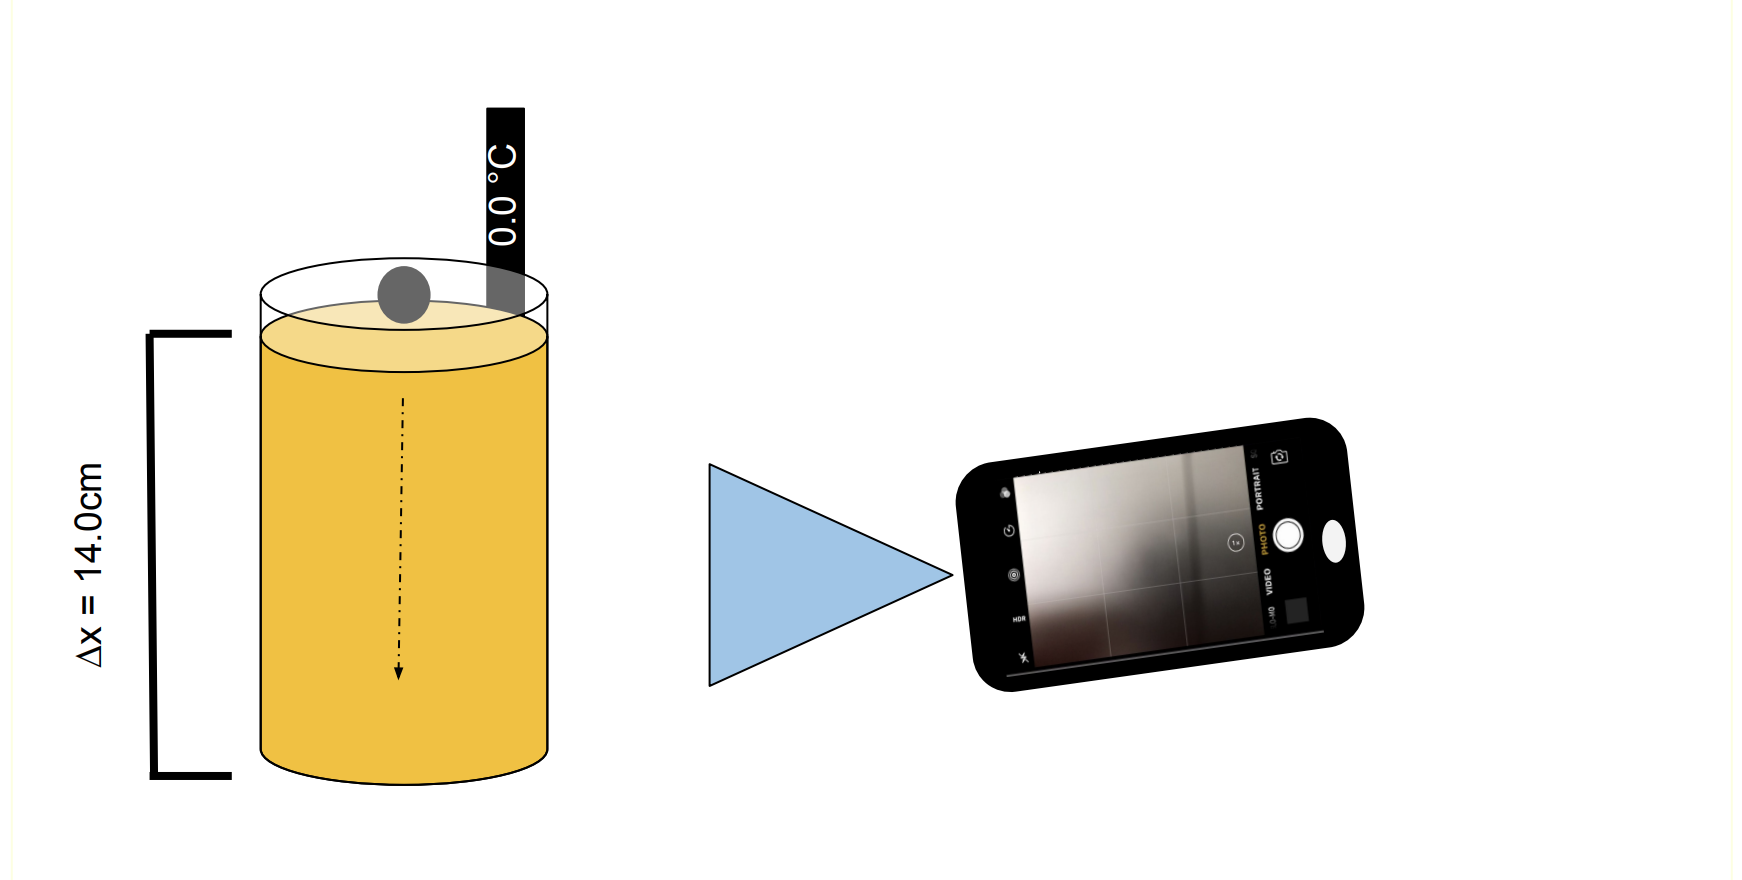
\includegraphics[width=3.0in]{schematic.png}
%
\caption{\label{setup} 
%Start with a clause summarizing what is presented in the figure.
Schematic of the ball drop and the measurement.
%Then add a sentence or two pointing out key features.
The canola oil is placed in a $14.0$ $cm$ tall cylindrical drinking glass. The marble is held above the canola oil, ready to drop. A thermometer is placed in the drinking glass.
A smartphone is placed adjacent to the glass, recording video.}
%
\end{figure}
%%%%%%%%%%%%%%%%%%%%Figure 1 end %%%%%%%%%%%%%%%%%%%%%%%

 %%%%%%%%%%%%%%%%%%%%Figure  2  begin %%%%%%%%%%%%%%%%%%%%%%%
\begin{figure}[t]
%
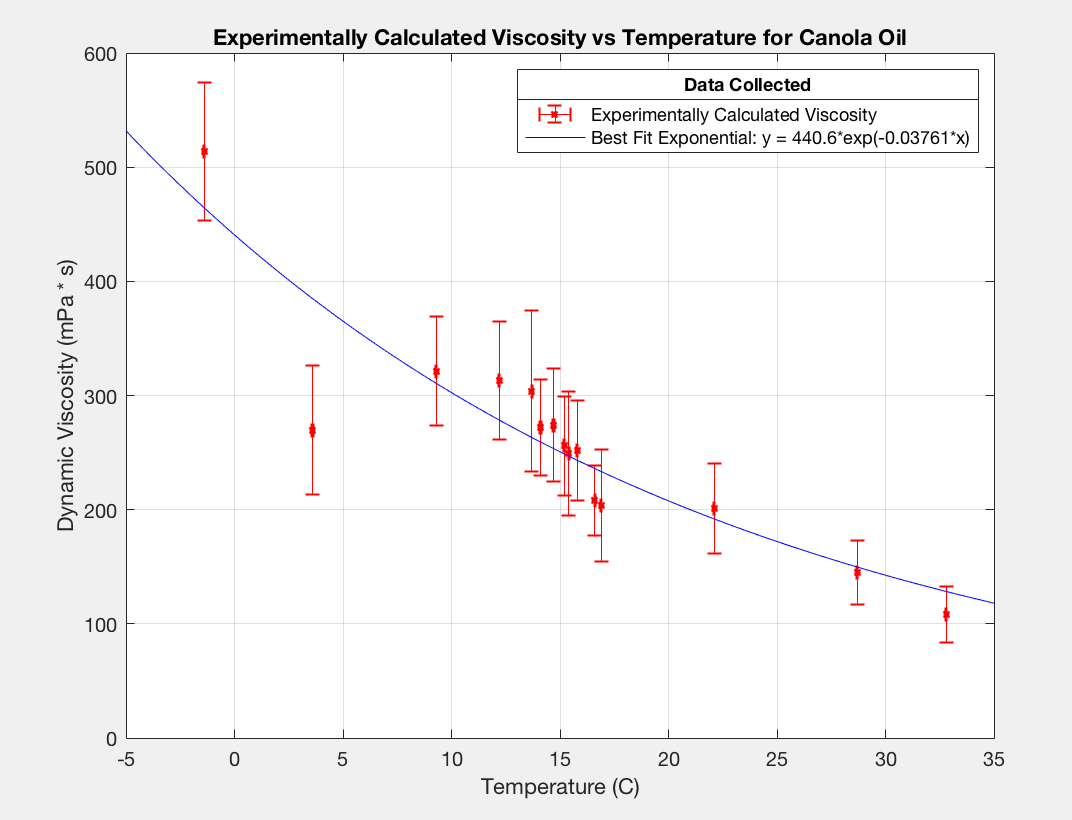
\includegraphics[width=3.0in]{graph1.png}
%
\caption{\label{graph} Graph of experimentally calculated data points for viscosity as a function of temperature, overlayed with the best fit exponential function. Error bars represent a 68$\%$ confidence interval.
}
%
\end{figure}
%%%%%%%%%%%%%%%%%%%% Figure  2  end %%%%%%%%%%%%%%%%%%%%%%%
% * <jamieclark.ast@gmail.com> 2018-05-31T04:53:40.673Z:
%
% ^.

%P7: Results 1 - Start by describing the raw data.  Raw data is what you directly measured, with no calculations or other processing. 
Data was processed using the programming language and development environment MATLAB\cite{MATLAB}, provided by licensing from the University of California, Santa Barbara. Graphs were also generated using MATLAB. Viscosity was calculated using Equation (\ref{eq4}), with our inputs being $m_{disp}$, $m$, $t$, $R$, and $\Delta x$, aswell as using the numerical constants $\pi$ and taking the accepted value of gravitational acceleration to be $g$ $=$ $9.80655 m/s^2$\cite{Gravity}. 

Viscosity was calculated for each individual temperature, and an exponential fit was applied to the data set.
Uncertainty in viscosity was derived from the uncertainty in the 5 measured quantities, and was propagated through using standard error propagation techniques involving adding in quadrature and partial differentiation\cite{ErrorPropagation}.
Uncertainty in the exponential fit was obtained from the curve-fitting software in MATLAB.

%P8: Results 2 - If you have two types of raw data, they may each require their own paragraph.  
%P9: Results 3 - Once you are done describing the raw data, then describe the measurement itself, making it clear what, if any, calculations were done.
Our measurements for time, viscosity, and their associated uncertainties can be viewed in Figure \ref{rawData3}.
Our raw data for viscosity as a function of temperature aswell as our exponential fit can be viewed graphically in Figure \ref{graph}.

Our exponential fit function for $\eta (T)$ is $\eta (T) = \alpha e^{-\beta T}$, where $\alpha = 440.65 \pm 30.40 \hspace{0.1cm} mPa\cdot s$ and $\beta = 0.03761 \hspace{0.1cm} \frac{1}{^{\circ}C}$. This fit resulted in an R-Square value of 0.8193 and an adjusted R-Square value of 0.8054. 

%%%%%%%%%%%%%%%%%%%% Figure 3 begin %%%%%%%%%%%%%%%%%%%%%%%
\begin{figure}[!h]
% TABLE HERE
\begin{center}
\begin{tabular}{ |c|c| } 
 \hline
Temperature$(^{\circ}$C) & Viscosity(mPa$\cdot$s) \\ 
 \hline
0 & 440.6482 $\pm$ 30.4047 \\
5 & 365.1094  $\pm$ 25.1925 \\
10 & 302.5199 $\pm$ 20.8739  \\
15 & 250.6599  $\pm$ 17.2955 \\
20 & 207.6901 $\pm$ 14.3306  \\
25 & 172.0864  $\pm$ 11.8740 \\
30 & 142.5862  $\pm$ 09.8384 \\




 \hline
\end{tabular}

\caption{\label{table1} Viscosity values generated via the Exponential Fit
}

\end{center}

\end{figure}

%%%%%%%%%%%%%%%%%%%% Figure 3 end %%%%%%%%%%%%%%%%%%%%%%%

%P10: Discussion - After presenting your result it is time to share any ideas you have about it. For example, you may want to say something about how your result compares with the results of others, published elsewhere.  Don't forget to  cite your sources!

It was difficult to find consistent results for the viscosity of canola oil, it is not the most common of experiments. One group of experimentalists, Diamante and Lan\cite{Diamante and Lan}, obtained a value of $46.2 mPa\cdot s \pm 0.5 mPa\cdot s$ at $30 ^{\circ}C$. 
This result is markedly lower than our result of $142.6 \pm 9.8$, and so I believe there may have been a systematic uncertainty in our measurement, perhaps due to constraints of the experiment, perhaps due to the constraints of the image analysis software. Additionally, the existence of a few outliers in our data, possibly due to the image analysis software, may have altered our result.


%P10:  Discussion - another good subject for discussion is your ideas for how the measurement approach could be improved.

Suggestions for a better experiment would include more resources. A taller container for the ball drop would be useful, so there is a lower relative uncertainty in the time data. A more precise scale to measure mass and more fine calipers to measure distance would also help diminish uncertainty.
The most important part to improve on would be the video analysis portion of the experiment. A larger container would allow for a longer video, which would be helpful for analysis. More sophisticated video analysis software would allow us to obtain a more precise measurement for position as a function of time, which would allow us to have more precise definitions for $v$ and $a$. We would be able to use $\frac{\partial^2 x}{\partial t^2}$ and $\frac{\partial x}{\partial t}$, as opposed to $<a>$ and $<v>$. 
This in particular might allow for diminished systematic error. 


%P11:  Discussion - use as many paragraphs as you like for the discussion.  It is fine to include matters of opinion, but be sure to support each assertion with clear reasoning. 



%P12:  Summary & Vision

In summary, we have measured the dynamic viscosity of canola oil as a function of temperature to be $\eta (T) = \alpha e^{-\beta T}$, where $\alpha = 440.65 \pm 30.40 \hspace{0.1cm} mPa\cdot s$ and $\beta = 0.03761 \hspace{0.1cm} \frac{1}{^{\circ}C}$.
Our measurement suffered errors due to the large uncertainty of some of the measurements, such as that of radius and mass. Our measurement also suffered from a lack of number of data points, I believe more trials on a larger range of temperatures could paint a clearer picture of how $\eta$ changes with temperature.
The most marked improvements to this approach would come from a larger set of data, more accurate measuring tools, and more sophisticated video analysis software.

%P21: Acknowledgements

I thank my lab partner, Evan Marschall for assistance in carrying out the experiment and for providing the materials for this lab, aswell as a place to do the experiment.  I am grateful to Joe Costello, Noah Swimmer, and Will Schultz for their assistance and mentorship in this experiment.  
This work was supported by Physics 25L lab fees.

\begin{thebibliography}{10}

\bibitem{Engines} Kopeliovich, Dmitri. $"$Effect of Oil Viscosity on Hydrodynamic Friction of Engine Bearings.$"$ SubsTech Substance and Technologies, 3 Feb. 2018. \url{http://www.substech.com/dokuwiki/doku.php?id=effect_of_oil_viscosity_on_hydrodynamic_friction_of_engine_bearings}

\bibitem{Chem_Book_Stokes_Drag} Laidler, Keith J.; Meiser, John H. (1982). Physical Chemistry. Benjamin/Cummings. p. 833. ISBN 0-8053-5682-7.

\bibitem{RHK} Halliday, David, et al. Physics. 5th ed., vol. 1, Wiley, 2002.

\bibitem{Footnote} Note that $m_{disp}$ refers to the mass of the displaced fluid.

\bibitem{canola_oil_density} "Section 3.1: Leaking Tank Experiments with Orimulsion and Canola Oil" (PDF). NOAA Technical Memorandum NOS OR$\&$R 6. Ocean Service of the National Oceanic and Atmospheric Administration. December 2001.

\bibitem{MATLAB} $"$MATLAB - MathWorks.$"$ MATLAB $\&$ Simulink, www.mathworks.com/products/matlab.html.

\bibitem{Gravity} Taylor, Barry N.; Thompson, Ambler, eds. (March 2008). The international system of units (SI) (pdf) (Report). National Institute of Standards and Technology. p. 52. NIST special publication 330, 2008 edition.

\bibitem{ErrorPropagation}  Ku, H. H. (October 1966). "Notes on the use of propagation of error formulas". Journal of Research of the National Bureau of Standards. National Bureau of Standards. 70C (4): 262. doi:10.6028/jres.070c.025. ISSN 0022-4316. Retrieved 3 October 2012.

\bibitem{Diamante and Lan} Lemuel M. Diamante and Tianying Lan, "Absolute Viscosities of Vegetable Oils at Different Temperatures and Shear Rate Range of 64.5 to 4835 s-1," Journal of Food Processing, vol. 2014, Article ID 234583, 6 pages, 2014. https://doi.org/10.1155/2014/234583.




\end{thebibliography}

\newpage

\begin{figure}
% TABLE HERE
\begin{center}
\begin{tabular}{ |c|c|c| } 
 \hline
Temperature$(^{\circ}$C) & Time(s) & Viscosity(mPa$\cdot$s) \\ 
 \hline
 -1.4  & 0.3685 $\pm$ 0.0144 & 513.92 $\pm$ 60.56 \\ 
 3.6 & 0.2778 $\pm$ 0.0164 & 269.65 $\pm$ 56.69 \\ 
9.3 & 0.2957 $\pm$ 0.0120 & 321.12 $\pm$ 47.82 \\ 
 12.2 & 0.2929 $\pm$ 0.0140 & 313.20 $\pm$ 51.75 \\ 
 13.7 & 0.2895 $\pm$ 0.0219 & 303.54 $\pm$ 70.49 \\ 
 14.1 & 0.2786 $\pm$ 0.0102 & 272.00 $\pm$ 42.43 \\ 
 14.7 & 0.2793 $\pm$ 0.0134 & 274.05 $\pm$ 49.52 \\ 
 15.2 & 0.2731 $\pm$ 0.0109 & 255.78 $\pm$ 43.41 \\ 
  15.4 & 0.2709 $\pm$ 0.0156 & 249.23 $\pm$ 54.57 \\ 
 15.8 & 0.2718 $\pm$ 0.0110 & 251.91 $\pm$ 43.52 \\ 
 16.6 & 0.2573 $\pm$ 0.0054 & 207.89 $\pm$ 30.45 \\ 
  16.9 & 0.2560 $\pm$ 0.0136 & 203.85 $\pm$ 49.20 \\ 
 22.1 & 0.2550 $\pm$ 0.0098 & 200.74 $\pm$ 39.44 \\ 
 28.7 & 0.2376 $\pm$ 0.0056 & 145.00 $\pm$ 27.94 \\ 
 32.8 & 0.2267 $\pm$ 0.0048 & 108.37 $\pm$ 24.76 \\ 




 \hline
\end{tabular}

\caption{\label{rawData3} List of measured times at each temperature, and calculated viscosity at each temperature. Other variables: $\Delta x = 14.0 cm \pm 0.0288 cm$, $R = 0.7 mm \pm 0.144mm$, $m = 5g \pm 0.288g$, $m_{disp}=1.3g \pm 0.086g$. 
}

\end{center}

\end{figure}

\end{document}
